%%% Econ714: Macroeconomics II
%%% Spring 2021
%%% Danny Edgel
%%%
% Due on Canvas Friday, April 23rd, 11:59pm Central Time
%%%

%%%
%							PREAMBLE
%%%

\documentclass{article}

%%% declare packages
\usepackage{amsmath}
\usepackage{amssymb}
\usepackage{array}
\usepackage{bm}
\usepackage{changepage}
\usepackage{centernot}
\usepackage{graphicx}
\usepackage{xcolor}
\usepackage[shortlabels]{enumitem}
\usepackage{fancyhdr}
	\fancyhf{} % sets both header and footer to nothing
	\renewcommand{\headrulewidth}{0pt}
    \rfoot{Edgel, \thepage}
    \pagestyle{fancy}
	
%%% define shortcuts for set notation
\newcommand{\Z}{\mathbb{Z}}
\newcommand{\R}{\mathbb{R}}
\newcommand{\Q}{\mathbb{Q}}
\newcommand{\lmt}{\underset{x\rightarrow\infty}{\text{lim }}}
\newcommand{\neglmt}{\underset{x\rightarrow-\infty}{\text{lim }}}
\newcommand{\zerolmt}{\underset{x\rightarrow 0}{\text{lim }}}
\newcommand{\loge}[1]{\text{log}\left(#1\right)}
\newcommand{\usmax}[1]{\underset{#1}{\text{max }}}
\newcommand{\usmin}[1]{\underset{#1}{\text{min }}}
\newcommand{\Mt}{M_{t+1}^t}
\newcommand{\vhat}{\hat{v}}
\newcommand{\olp}{\overline{p}}
\renewcommand{\L}{\mathcal{L}}
\newcommand{\olq}{\overline{q}}
\newcommand{\zinf}{_{t=0}^\infty}
\newcommand{\aneg}{A^{-1}}
\newcommand{\sneg}{s^{-1}}
\newcommand{\olk}{\overline{k}}
\newcommand{\olc}{\overline{c}}
\newcommand{\olr}{\overline{r}}
\newcommand{\olpi}{\overline{\pi}}
\newcommand{\Aneg}{A^{-1}}
\renewcommand{\sneg}{s^{-1}}
\newcommand{\dc}[1]{\Delta c_{#1}}
\newcommand{\N}{\mathcal{N}}
\newcommand{\suminf}{\sum_{t=0}^\infty}
\newcommand{\sumn}{\sum_{i=1}^{n}}
\newcommand{\sumnk}{\sum_{i=1}^{N_k}}
\newcommand{\red}[1]{{\color{red}#1}}
\newcommand{\Tau}{\mathrm{T}}
\newcommand{\phat}{\hat{p}}

\newcommand{\E}[1]{\mathbb{E}\left[#1\right]} % expected value
\newcommand{\Et}[1]{\mathbb{E}_t\left[#1\right]}

%%% define column vector command (from Michael Nattinger)
\newcount\colveccount
\newcommand*\colvec[1]{
        \global\colveccount#1
        \begin{pmatrix}
        \colvecnext
}
\def\colvecnext#1{
        #1
        \global\advance\colveccount-1
        \ifnum\colveccount>0
                \\
                \expandafter\colvecnext
        \else
                \end{pmatrix}
        \fi
}

%%% define function for drawing matrix augmentation lines
\newcommand\aug{\fboxsep=-\fboxrule\!\!\!\fbox{\strut}\!\!\!}

\makeatletter
\let\amsmath@bigm\bigm

\renewcommand{\bigm}[1]{%
  \ifcsname fenced@\string#1\endcsname
    \expandafter\@firstoftwo
  \else
    \expandafter\@secondoftwo
  \fi
  {\expandafter\amsmath@bigm\csname fenced@\string#1\endcsname}%
  {\amsmath@bigm#1}%
}


%________________________________________________________________%

\begin{document}

\title{	Problem Set \#1 }
\author{ 		Danny Edgel 						\\ 
			Econ 899: Computational Methods		\\
			Fall 2021						\\
		}
\maketitle\thispagestyle{empty}


%%%________________________________________________________________%%%

\begin{enumerate}
	% State the dynamic programming problem
	\item The dynamic programming problem is:
	\[
		\usmax{\left\{K_{t+1}, C_t\right\}_{t=1}^\infty}\E{\sum_{t=1}^\infty\beta^t\loge{C_t}}
			\text{ s.t. }C_t + K_{t+1} - (1-\delta)K_t\leq Z_tK_t^\theta\text{ }\forall t = 1,2,3,...
	\]
	Which can be represented by the following Bellman equation:
	\[
		V(K,Z) = \usmax{K'}\left\{\loge{ZK^\theta + (1-\delta)K - K'} + \beta\E{V(K', Z)|Z}\right\}
	\]
	I did not complete the programming exercise in Fortran, but I completed it in Julia, both parallelized and not (see edgel\_ps1.jl, edgel\_growth\_model.jl, edgel\_ps1\_unparrallel.jl, and edgel\_growth\_model\_unparrallel.jl). For the timing comparison, I asked Michell Vald\'{e}z Bobes for his Fortran times. The timing comparisons are provided below, for unparallelized code, code that parallelizes the state space loop, and code that parallelizes the capital state space loop.
	\begin{center}
		\begin{tabular}{r|ccc}
					& Unparallelized	& Parallelized, $Z$	& Parallelized, $K$	\\\hline
			Julia		& 13.63		& 15.38		& 14.02		\\
			Fortran 	& 15.35		& 4.71		& \textit{N/A}
		\end{tabular}
	\end{center}
	
	% Plot the value frunction over K for each state Z. Is it increasing? Is it concave?
	\item The value function for each state, $Z$, is plotted below. For each state, the value function is clearly both increasing and concave.
	\begin{center}
		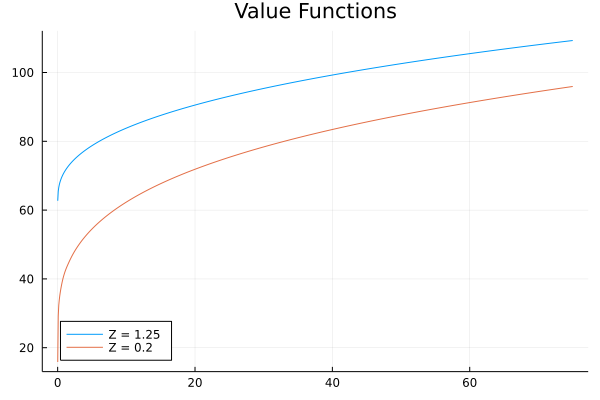
\includegraphics[scale=.55]{02_Value_Functions.png}
	\end{center}
	
	% Is the decision rule increasing in K and Z? Is saving increasing in K and Z?
	\item The policy function for each state is displayed below, and the decision rule is clearly increasing in both $K$ and $Z$, as is saving.
	\begin{center}
		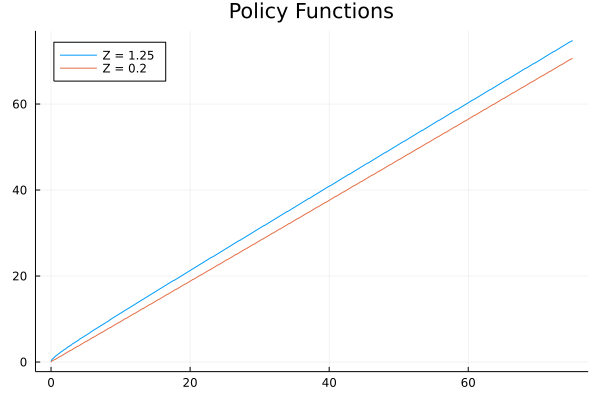
\includegraphics[scale=.55]{02_Policy_Functions.png}
	\end{center}
	
	% Compare speed savings from parallel computing!
\end{enumerate}

%%%________________________________________________________________%%%




\end{document}






